% Options for packages loaded elsewhere
\PassOptionsToPackage{unicode}{hyperref}
\PassOptionsToPackage{hyphens}{url}
%
\documentclass[
]{article}
\usepackage{amsmath,amssymb}
\usepackage{lmodern}
\usepackage{iftex}
\ifPDFTeX
  \usepackage[T1]{fontenc}
  \usepackage[utf8]{inputenc}
  \usepackage{textcomp} % provide euro and other symbols
\else % if luatex or xetex
  \usepackage{unicode-math}
  \defaultfontfeatures{Scale=MatchLowercase}
  \defaultfontfeatures[\rmfamily]{Ligatures=TeX,Scale=1}
\fi
% Use upquote if available, for straight quotes in verbatim environments
\IfFileExists{upquote.sty}{\usepackage{upquote}}{}
\IfFileExists{microtype.sty}{% use microtype if available
  \usepackage[]{microtype}
  \UseMicrotypeSet[protrusion]{basicmath} % disable protrusion for tt fonts
}{}
\makeatletter
\@ifundefined{KOMAClassName}{% if non-KOMA class
  \IfFileExists{parskip.sty}{%
    \usepackage{parskip}
  }{% else
    \setlength{\parindent}{0pt}
    \setlength{\parskip}{6pt plus 2pt minus 1pt}}
}{% if KOMA class
  \KOMAoptions{parskip=half}}
\makeatother
\usepackage{xcolor}
\IfFileExists{xurl.sty}{\usepackage{xurl}}{} % add URL line breaks if available
\IfFileExists{bookmark.sty}{\usepackage{bookmark}}{\usepackage{hyperref}}
\hypersetup{
  hidelinks,
  pdfcreator={LaTeX via pandoc}}
\urlstyle{same} % disable monospaced font for URLs
\usepackage[left=1.1cm,right=1.1cm,top=1.75cm,bottom=1.75cm]{geometry}
\usepackage{color}
\usepackage{fancyvrb}
\newcommand{\VerbBar}{|}
\newcommand{\VERB}{\Verb[commandchars=\\\{\}]}
\DefineVerbatimEnvironment{Highlighting}{Verbatim}{commandchars=\\\{\}}
% Add ',fontsize=\small' for more characters per line
\usepackage{framed}
\definecolor{shadecolor}{RGB}{248,248,248}
\newenvironment{Shaded}{\begin{snugshade}}{\end{snugshade}}
\newcommand{\AlertTok}[1]{\textcolor[rgb]{0.94,0.16,0.16}{#1}}
\newcommand{\AnnotationTok}[1]{\textcolor[rgb]{0.56,0.35,0.01}{\textbf{\textit{#1}}}}
\newcommand{\AttributeTok}[1]{\textcolor[rgb]{0.77,0.63,0.00}{#1}}
\newcommand{\BaseNTok}[1]{\textcolor[rgb]{0.00,0.00,0.81}{#1}}
\newcommand{\BuiltInTok}[1]{#1}
\newcommand{\CharTok}[1]{\textcolor[rgb]{0.31,0.60,0.02}{#1}}
\newcommand{\CommentTok}[1]{\textcolor[rgb]{0.56,0.35,0.01}{\textit{#1}}}
\newcommand{\CommentVarTok}[1]{\textcolor[rgb]{0.56,0.35,0.01}{\textbf{\textit{#1}}}}
\newcommand{\ConstantTok}[1]{\textcolor[rgb]{0.00,0.00,0.00}{#1}}
\newcommand{\ControlFlowTok}[1]{\textcolor[rgb]{0.13,0.29,0.53}{\textbf{#1}}}
\newcommand{\DataTypeTok}[1]{\textcolor[rgb]{0.13,0.29,0.53}{#1}}
\newcommand{\DecValTok}[1]{\textcolor[rgb]{0.00,0.00,0.81}{#1}}
\newcommand{\DocumentationTok}[1]{\textcolor[rgb]{0.56,0.35,0.01}{\textbf{\textit{#1}}}}
\newcommand{\ErrorTok}[1]{\textcolor[rgb]{0.64,0.00,0.00}{\textbf{#1}}}
\newcommand{\ExtensionTok}[1]{#1}
\newcommand{\FloatTok}[1]{\textcolor[rgb]{0.00,0.00,0.81}{#1}}
\newcommand{\FunctionTok}[1]{\textcolor[rgb]{0.00,0.00,0.00}{#1}}
\newcommand{\ImportTok}[1]{#1}
\newcommand{\InformationTok}[1]{\textcolor[rgb]{0.56,0.35,0.01}{\textbf{\textit{#1}}}}
\newcommand{\KeywordTok}[1]{\textcolor[rgb]{0.13,0.29,0.53}{\textbf{#1}}}
\newcommand{\NormalTok}[1]{#1}
\newcommand{\OperatorTok}[1]{\textcolor[rgb]{0.81,0.36,0.00}{\textbf{#1}}}
\newcommand{\OtherTok}[1]{\textcolor[rgb]{0.56,0.35,0.01}{#1}}
\newcommand{\PreprocessorTok}[1]{\textcolor[rgb]{0.56,0.35,0.01}{\textit{#1}}}
\newcommand{\RegionMarkerTok}[1]{#1}
\newcommand{\SpecialCharTok}[1]{\textcolor[rgb]{0.00,0.00,0.00}{#1}}
\newcommand{\SpecialStringTok}[1]{\textcolor[rgb]{0.31,0.60,0.02}{#1}}
\newcommand{\StringTok}[1]{\textcolor[rgb]{0.31,0.60,0.02}{#1}}
\newcommand{\VariableTok}[1]{\textcolor[rgb]{0.00,0.00,0.00}{#1}}
\newcommand{\VerbatimStringTok}[1]{\textcolor[rgb]{0.31,0.60,0.02}{#1}}
\newcommand{\WarningTok}[1]{\textcolor[rgb]{0.56,0.35,0.01}{\textbf{\textit{#1}}}}
\usepackage{graphicx}
\makeatletter
\def\maxwidth{\ifdim\Gin@nat@width>\linewidth\linewidth\else\Gin@nat@width\fi}
\def\maxheight{\ifdim\Gin@nat@height>\textheight\textheight\else\Gin@nat@height\fi}
\makeatother
% Scale images if necessary, so that they will not overflow the page
% margins by default, and it is still possible to overwrite the defaults
% using explicit options in \includegraphics[width, height, ...]{}
\setkeys{Gin}{width=\maxwidth,height=\maxheight,keepaspectratio}
% Set default figure placement to htbp
\makeatletter
\def\fps@figure{htbp}
\makeatother
\setlength{\emergencystretch}{3em} % prevent overfull lines
\providecommand{\tightlist}{%
  \setlength{\itemsep}{0pt}\setlength{\parskip}{0pt}}
\setcounter{secnumdepth}{-\maxdimen} % remove section numbering
\usepackage{fancyhdr}
\ifLuaTeX
  \usepackage{selnolig}  % disable illegal ligatures
\fi

\title{Lista de Exercícios II - Bioestatística (DES4060 - Turma 2022)}
\author{Prof.: Dr.~Robson Marcelo Rossi \and Aluno: João Matheus Slujala
Krüger Taborda Hneda}
\date{}

\begin{document}
\maketitle

\renewcommand*\contentsname{Sumário}
{
\setcounter{tocdepth}{5}
\tableofcontents
}
\newpage

\hypertarget{especificauxe7uxf5es}{%
\section{Especificações}\label{especificauxe7uxf5es}}

Encontrar alguma distribuição de probabilidade nova (pelo menos 2
parâmetros) e:

\begin{itemize}
\tightlist
\item
  escrever quem fez, onde usou, como usou, propriedades
\item
  implementar as funções d, p, q r
\item
  fazer figuras
\item
  realizar estudo de simulação (estimação máxima verossimilhança) --
  variar tamanho da amostra e ver como as estimativas mudam, viés, rmse
\end{itemize}

\hypertarget{escrever-quem-fez-onde-usou-como-usou-propriedades}{%
\section{escrever quem fez, onde usou, como usou,
propriedades}\label{escrever-quem-fez-onde-usou-como-usou-propriedades}}

\hypertarget{implementar-as-funuxe7uxf5es-p-d-q-r}{%
\section{implementar as funções p, d, q,
r}\label{implementar-as-funuxe7uxf5es-p-d-q-r}}

\begin{Shaded}
\begin{Highlighting}[]
\FunctionTok{graphics.off}\NormalTok{()}
\DocumentationTok{\#\#\#\#\#\#\#\#\#\#\#\#\#\#\#\#\#\#\#\#\#\#\#\#\#\#\#\#\#\#\#\#\#\#\#\#\#\#\#\#\#\#\#\#\#\#\#\#\#\#\#\#\#\#\#\#\#\#\#\#\#\#\#\#\#\#\#\#\#\#\#\#\#\#\#\#\#\#\#}
\NormalTok{pgenhalf }\OtherTok{\textless{}{-}} \ControlFlowTok{function}\NormalTok{(q, theta, alpha)}
\NormalTok{\{}
  \DecValTok{2} \SpecialCharTok{*} \FunctionTok{pnorm}\NormalTok{((q }\SpecialCharTok{/}\NormalTok{ theta) }\SpecialCharTok{\^{}}\NormalTok{ alpha) }\SpecialCharTok{{-}} \DecValTok{1}
\NormalTok{\}}
\end{Highlighting}
\end{Shaded}

\begin{Shaded}
\begin{Highlighting}[]
\DocumentationTok{\#\#\#\#\#\#\#\#\#\#\#\#\#\#\#\#\#\#\#\#\#\#\#\#\#\#\#\#\#\#\#\#\#\#\#\#\#\#\#\#\#\#\#\#\#\#\#\#\#\#\#\#\#\#\#\#\#\#\#\#\#\#\#\#\#\#\#\#\#\#\#\#\#\#\#\#\#\#\#\#}
\NormalTok{dgenhalf }\OtherTok{\textless{}{-}} \ControlFlowTok{function}\NormalTok{(x, theta, alpha)}
\NormalTok{\{}
\NormalTok{  xtheta }\OtherTok{\textless{}{-}}\NormalTok{ (x }\SpecialCharTok{/}\NormalTok{ theta) }\SpecialCharTok{\^{}}\NormalTok{ alpha}
  \FunctionTok{sqrt}\NormalTok{(}\DecValTok{2} \SpecialCharTok{/}\NormalTok{ pi) }\SpecialCharTok{*}\NormalTok{ (alpha }\SpecialCharTok{/}\NormalTok{ x) }\SpecialCharTok{*}\NormalTok{ xtheta  }\SpecialCharTok{*} \FunctionTok{exp}\NormalTok{(}\SpecialCharTok{{-}}\FloatTok{0.5} \SpecialCharTok{*}\NormalTok{ xtheta }\SpecialCharTok{\^{}} \DecValTok{2}\NormalTok{)}
\NormalTok{\}}
\end{Highlighting}
\end{Shaded}

\begin{Shaded}
\begin{Highlighting}[]
\DocumentationTok{\#\#\#\#\#\#\#\#\#\#\#\#\#\#\#\#\#\#\#\#\#\#\#\#\#\#\#\#\#\#\#\#\#\#\#\#\#\#\#\#\#\#\#\#\#\#\#\#\#\#\#\#\#\#\#\#\#\#\#\#\#\#\#\#\#\#\#\#\#\#\#\#\#\#\#\#\#\#\#\#}
\NormalTok{qgenhalf }\OtherTok{\textless{}{-}} \ControlFlowTok{function}\NormalTok{(p, theta, alpha)}
\NormalTok{\{}
\NormalTok{  theta }\SpecialCharTok{*} \FunctionTok{qnorm}\NormalTok{((p }\SpecialCharTok{+} \DecValTok{1}\NormalTok{) }\SpecialCharTok{*} \FloatTok{0.5}\NormalTok{) }\SpecialCharTok{\^{}}\NormalTok{ (}\DecValTok{1} \SpecialCharTok{/}\NormalTok{ alpha)}
\NormalTok{\}}
\end{Highlighting}
\end{Shaded}

\begin{Shaded}
\begin{Highlighting}[]
\DocumentationTok{\#\#\#\#\#\#\#\#\#\#\#\#\#\#\#\#\#\#\#\#\#\#\#\#\#\#\#\#\#\#\#\#\#\#\#\#\#\#\#\#\#\#\#\#\#\#\#\#\#\#\#\#\#\#\#\#\#\#\#\#\#\#\#\#\#\#\#\#\#\#\#\#\#\#\#\#\#\#\#\#}
\NormalTok{rgenhalf }\OtherTok{\textless{}{-}} \ControlFlowTok{function}\NormalTok{(n, theta, alpha)}
\NormalTok{\{}
\NormalTok{  U }\OtherTok{\textless{}{-}} \FunctionTok{runif}\NormalTok{(n)}
\NormalTok{  theta }\SpecialCharTok{*} \FunctionTok{qnorm}\NormalTok{((U }\SpecialCharTok{+} \DecValTok{1}\NormalTok{) }\SpecialCharTok{*} \FloatTok{0.5}\NormalTok{) }\SpecialCharTok{\^{}}\NormalTok{ (}\DecValTok{1} \SpecialCharTok{/}\NormalTok{ alpha)}
\NormalTok{\}}
\DocumentationTok{\#\#\#\#\#\#\#\#\#\#\#\#\#\#\#\#\#\#\#\#\#\#\#\#\#\#\#\#\#\#\#\#\#\#\#\#\#\#\#\#\#\#\#\#\#\#\#\#\#\#\#\#\#\#\#\#\#\#\#\#\#\#\#\#\#\#\#\#\#\#\#\#\#\#\#\#\#\#\#\#}
\end{Highlighting}
\end{Shaded}

\begin{Shaded}
\begin{Highlighting}[]
\NormalTok{x }\OtherTok{\textless{}{-}} \FunctionTok{rgenhalf}\NormalTok{(}\DecValTok{10000}\NormalTok{, }\AttributeTok{theta =} \DecValTok{4}\NormalTok{, }\AttributeTok{alpha =} \DecValTok{3}\NormalTok{)}
\FunctionTok{x11}\NormalTok{(); }\FunctionTok{hist}\NormalTok{(x, }\AttributeTok{prob =}\NormalTok{ T)}
\NormalTok{y }\OtherTok{\textless{}{-}} \FunctionTok{seq}\NormalTok{(}\FloatTok{0.1}\NormalTok{, }\DecValTok{100}\NormalTok{, }\FloatTok{0.0001}\NormalTok{)}
\FunctionTok{lines}\NormalTok{(y, }\FunctionTok{dgenhalf}\NormalTok{(y, }\AttributeTok{theta =} \DecValTok{4}\NormalTok{, }\AttributeTok{alpha =} \DecValTok{3}\NormalTok{), }\AttributeTok{lwd =} \DecValTok{2}\NormalTok{, }\AttributeTok{col =} \StringTok{"red"}\NormalTok{)}
\end{Highlighting}
\end{Shaded}

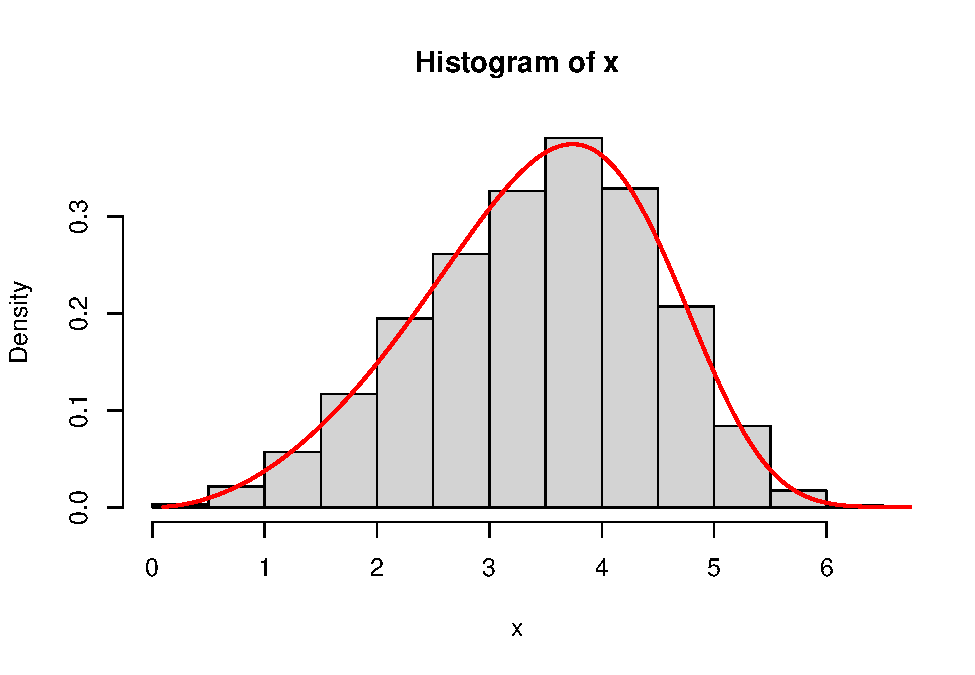
\includegraphics{code_files/figure-latex/unnamed-chunk-5-1.pdf}

\hypertarget{fazer-figuras}{%
\section{fazer figuras}\label{fazer-figuras}}

\end{document}
